\chapter{Metodologia}

\section{Questões de Pesquisa e Abordagem}
Este capítulo descreve o desenho experimental que operacionaliza as questões
de pesquisa que orientam este trabalho. A questão
principal investiga como a eficácia de diferentes estratégias de
retreinamento varia em função do tipo, entendido como padrão temporal, da
severidade do drift enfrentado e do classificador monitorado. A questão
derivada investiga, de forma exploratória, se sinais observáveis do detector
permitem esboçar uma orientação de escolha de estratégia aplicável a
produção.

Responder a essas questões exige conhecer, para cada observação, o tipo e a
severidade reais do drift enfrentado, informação que, em dados reais de
produção, nunca está disponível, precisamente porque o tipo e a severidade
verdadeiros são características latentes (Seção~\ref{sec:sinais}). Por isso,
este trabalho adota uma abordagem experimental quantitativa, e não um estudo
observacional sobre dados de produção: apenas um ambiente controlado, no
qual o próprio pesquisador injeta o drift e, portanto, conhece o ground
truth de tipo e severidade, permite isolar o efeito de cada uma dessas
variáveis sobre a eficácia da estratégia, algo que um estudo observacional,
limitado a inferir o tipo de drift de forma indireta, não permitiria fazer
com o mesmo rigor causal.

Dentro da abordagem experimental, a escolha por um desenho fatorial
(Seção~\ref{sec:fatorial}), em vez de comparações par a par entre
estratégias, se justifica pela própria formulação da questão principal: como
ela pergunta simultaneamente sobre a variação da eficácia em função de tipo,
severidade e classificador, e sobre a interação conjunta entre essas três
variáveis, um desenho fatorial completo é a única forma de estimar tanto os
efeitos principais quanto as interações entre os três fatores na mesma
bateria de execuções. O ambiente de stream, por sua vez, é o que possibilita
testar a questão derivada: como
o desdobramento exploratório depende da comparação entre sinais observáveis
pelo detector, calculados de forma incremental sobre janelas sucessivas de
uma stream, e o ground truth conhecido por injeção, um cenário de batch
estático não permitiria gerar esses sinais da mesma forma como estariam
disponíveis em produção real. A abordagem é, portanto, experimental e
quantitativa: um experimento fatorial controlado, executado sobre streams
sintéticas nas quais tipo e severidade do drift são conhecidos por injeção
(Seção~\ref{sec:severidade}), com o HDDDM mantido fixo como mecanismo de
detecção em todas as condições (Seção~\ref{sec:deteccao}). A
Figura~\ref{fig:fluxo_geral} apresenta uma visão geral desse fluxo antes do
detalhamento de cada etapa nas seções seguintes.

\begin{figure}[h]
\centering
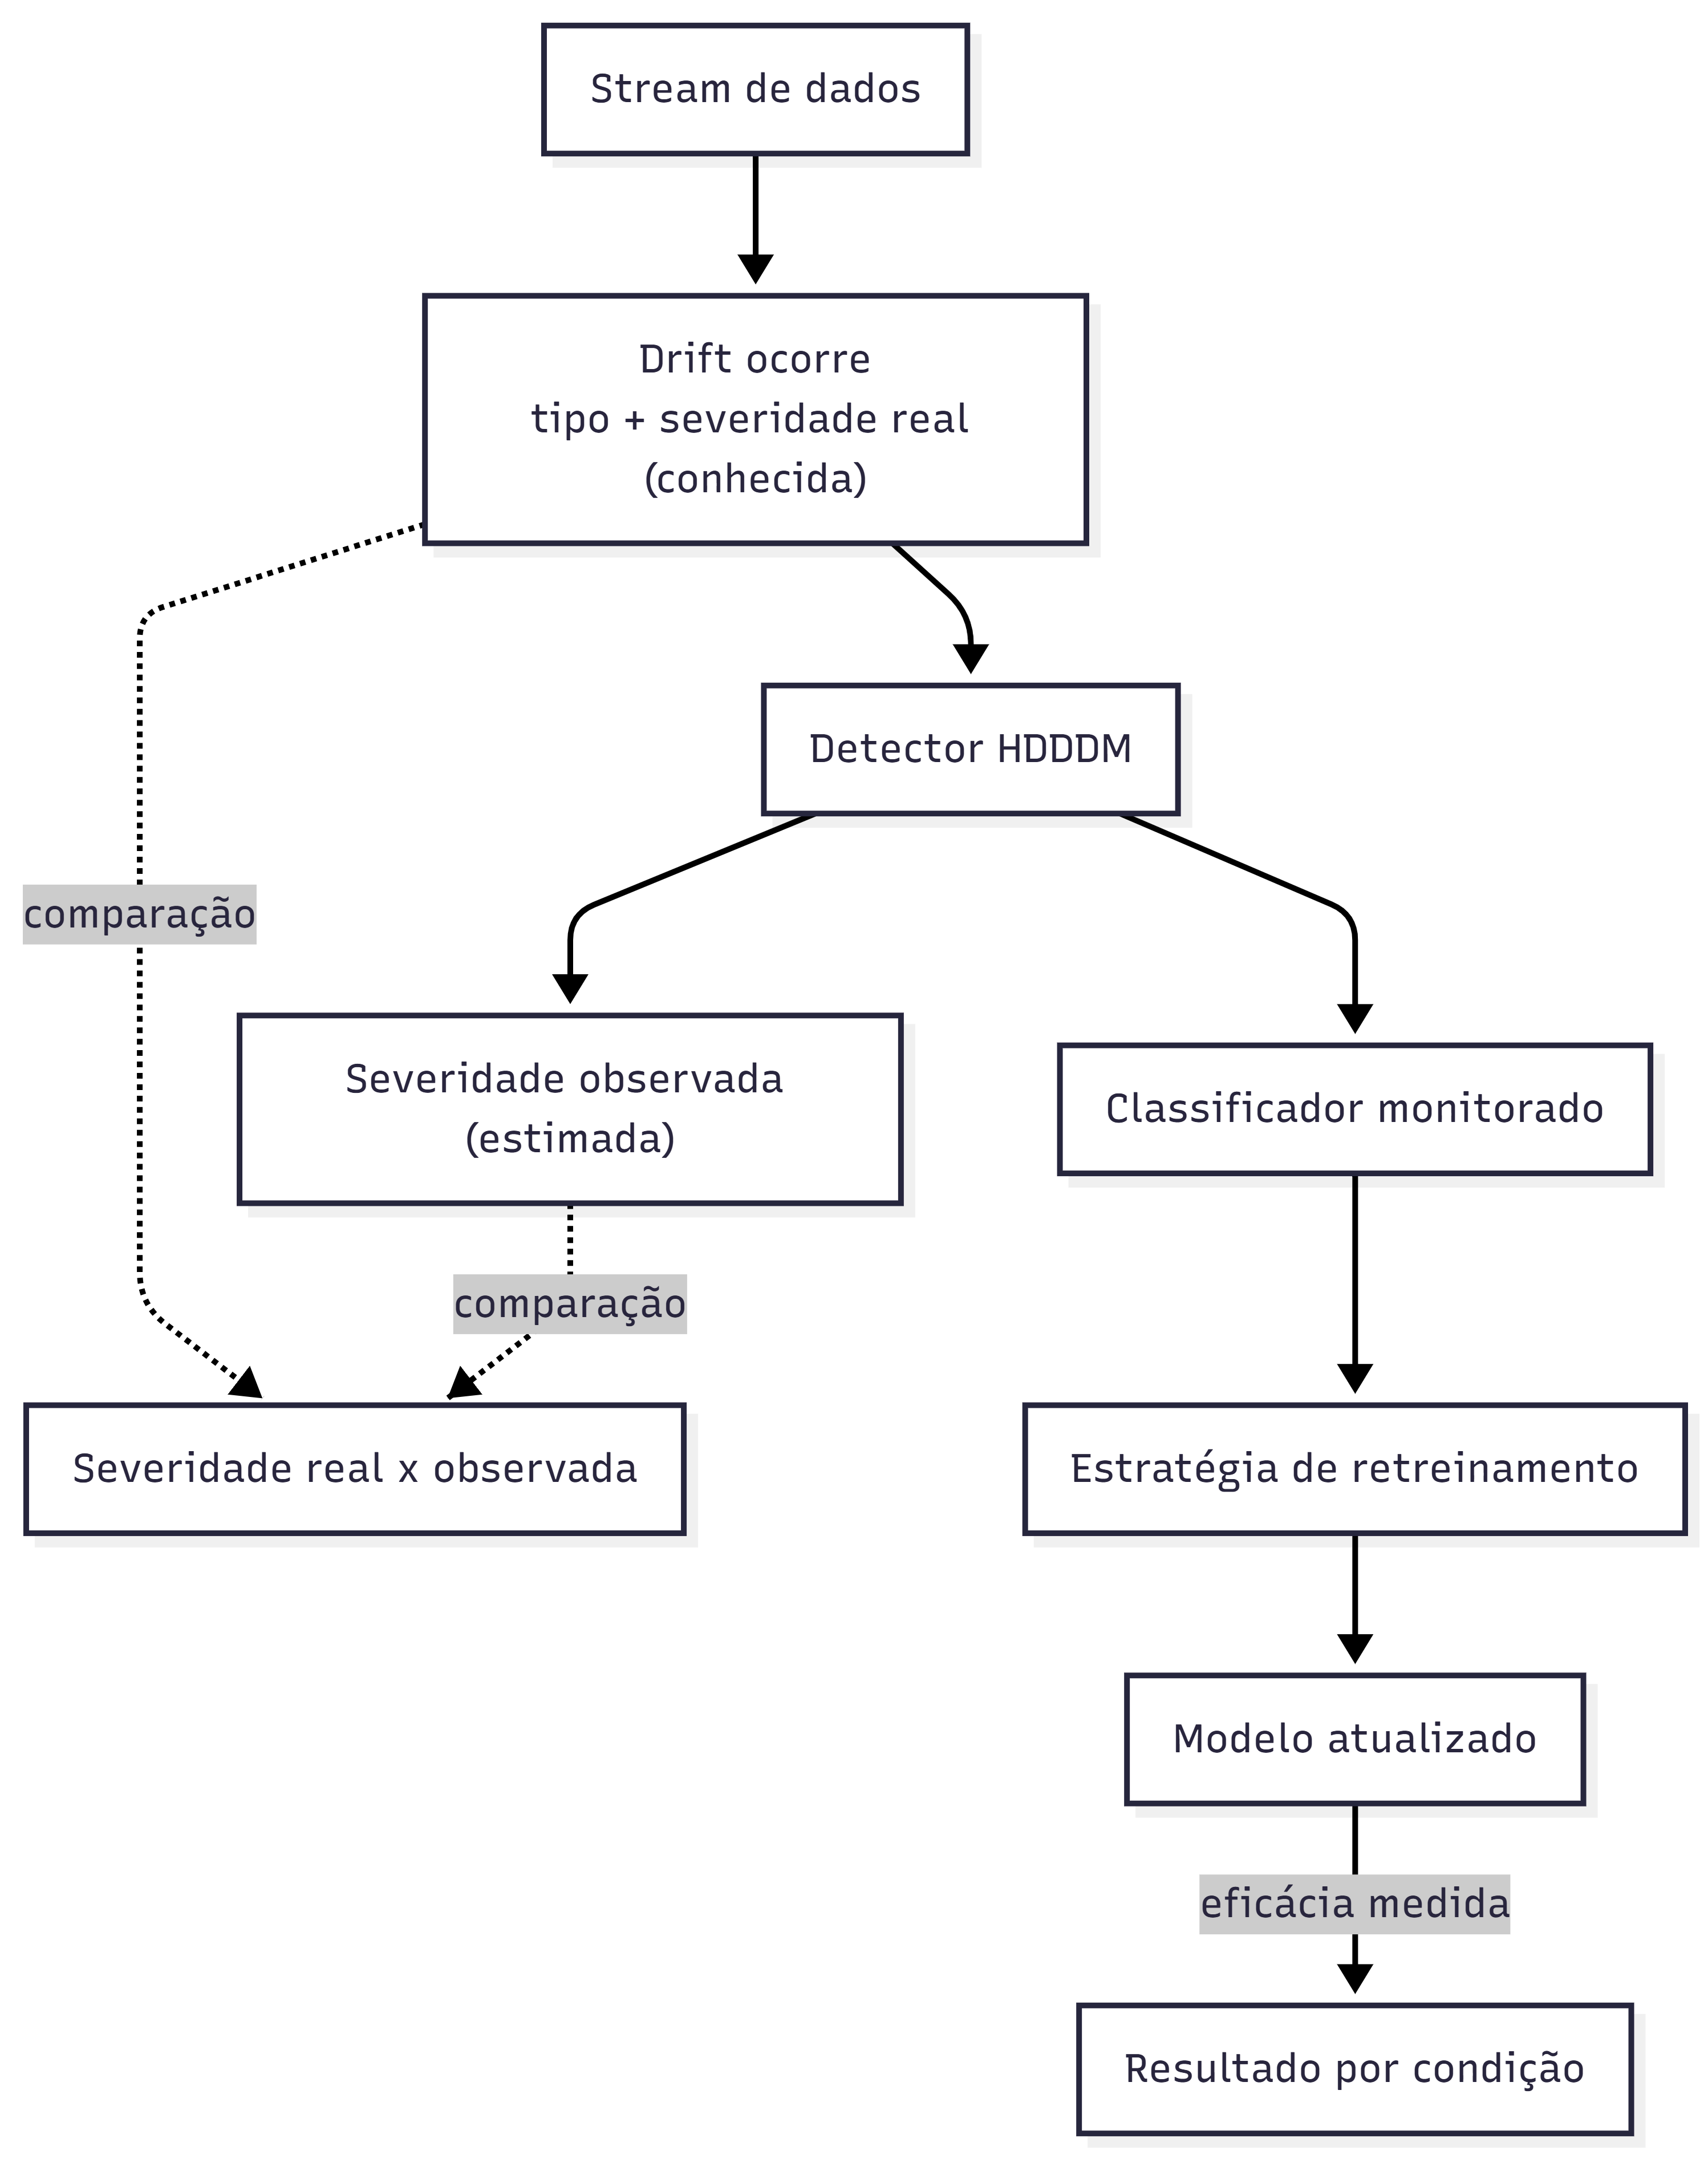
\includegraphics[width=0.5\textwidth]{figuras/fluxo.png}
\caption{Visão geral do fluxo experimental: o fluxo principal vai da stream
de dados ao resultado por condição; a severidade real, conhecida por
injeção, e a severidade observada, estimada pelo detector, convergem numa
comparação que fundamenta a questão derivada.}
\label{fig:fluxo_geral}
\end{figure}

\section{Geração da Stream Sintética}
\label{sec:geracao_stream}
Cada stream é uma sequência de instâncias rotuladas, geradas a partir de uma
distribuição base que permanece estável até o ponto de injeção do drift.
Sobre essa base, os quatro padrões temporais definidos na
Seção~\ref{sec:severidade} são operacionalizados como segue, todos
parametrizados pelo mesmo deslocamento padronizado $\Delta/\sigma$ associado
ao nível de severidade da condição:

\begin{itemize}
  \item \textbf{Abrupto}: a distribuição muda de $P$ para $Q$ em uma única
  instância de transição, sem período intermediário.
  \item \textbf{Gradual}: durante uma janela de transição de largura fixa,
  cada nova instância é sorteada de $P$ ou $Q$ com probabilidade que se
  desloca linearmente de 0 a 1 ao longo da janela, de modo que $Q$ passe a
  predominar ao final da transição.
  \item \textbf{Incremental}: o deslocamento total $\Delta$ é dividido em
  pequenos incrementos aplicados a cada bloco de instâncias ao longo da
  janela de transição, de modo que a distribuição se mova continuamente de
  $P$ a $Q$ sem alternância entre estados.
  \item \textbf{Recorrente}: a distribuição alterna entre três estados
  ($P$, $Q$, $R$) ao longo de intervalos fixos, na sequência $P \to Q \to R
  \to P$, cada transição caracterizada pelo mesmo deslocamento padronizado
  $\Delta/\sigma$ em relação ao estado imediatamente anterior. Alternar
  entre mais de dois estados garante que, quando $P$ reaparece, o
  repositório de modelos descartados (Seção~\ref{sec:estrategias}) já
  contenha ao menos dois candidatos distintos, os modelos treinados sob
  $Q$ e sob $R$, permitindo testar de fato a seleção do candidato mais
  próximo por distância de Hellinger, e não apenas a reativação de um único
  modelo historicamente possível.
\end{itemize}

Em todos os quatro padrões, a severidade nominal da condição corresponde ao
$\Delta/\sigma$ definido para o deslocamento completo entre estados
consecutivos (Equação~\ref{eq:severidade}); os padrões gradual e incremental
diferem apenas na trajetória percorrida até esse deslocamento, não no seu
valor final. A Figura~\ref{fig:padroes_temporais} ilustra os quatro padrões
como séries temporais simplificadas.

\begin{figure}[h]
\centering
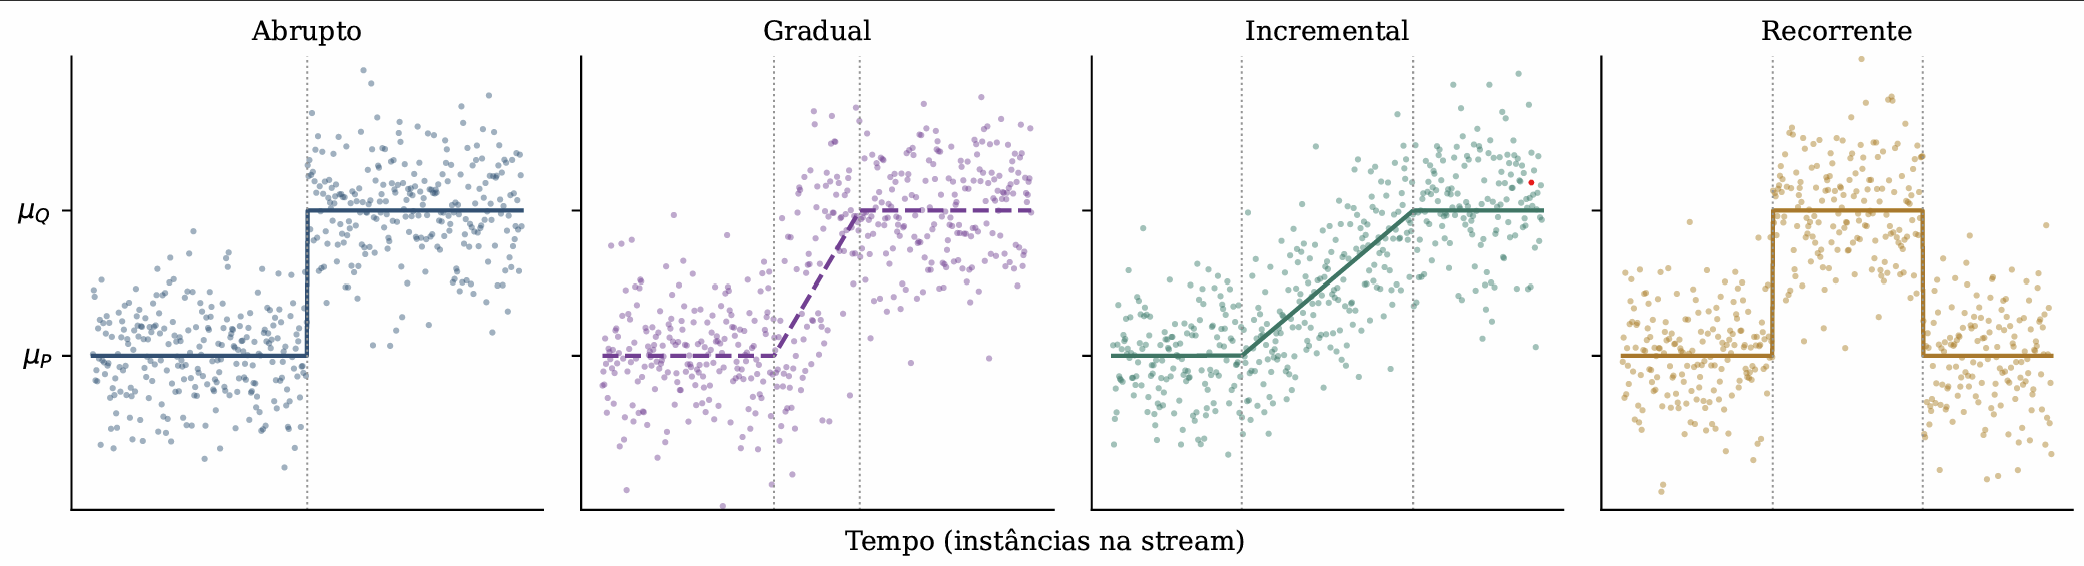
\includegraphics[keepaspectratio=true,scale=0.5]{figuras/padrao_temporal.png}
\caption{Os quatro padrões temporais de drift operacionalizados na geração
da stream sintética, mostrando a transição entre a distribuição $P$
(pré-drift) e $Q$ (pós-drift) ao longo do tempo.}
\label{fig:padroes_temporais}
\end{figure}

\section{Classificadores e Adaptação a Stream}
Os três classificadores descritos na Seção de Classificadores do referencial
teórico permanecem, entre atualizações, congelados no estado em que foram
treinados pela última vez; nenhum deles se atualiza continuamente por
exigência própria. O Naive Bayes atualiza contadores de forma nativa e
imediata; o Random Forest, na variante adaptativa discutida por
\citeonline{gomes2017}, mantém um conjunto de árvores substituíveis; o
XGBoost mantém o conjunto de árvores já construído e só o modifica quando
uma estratégia de retreinamento é efetivamente acionada. Essa uniformidade é
deliberada: ela garante que a variável manipulada seja a estratégia de
retreinamento, e não uma exigência de atualização embutida em um classificador
específico; em particular, a adaptação de XGBoost a stream via lotes
pequenos (referencial teórico, Seção de Classificadores) descreve apenas
\emph{como} uma atualização é executada quando decidida, não uma atualização
contínua imposta pelo classificador.

\section{Estratégias de Retreinamento: Operacionalização}
As quatro estratégias definidas no referencial teórico, mais a condição de
controle, são operacionalizadas de forma uniforme entre classificadores,
variando apenas o procedimento técnico de ajuste de parâmetros:

\begin{itemize}
  \item \textbf{Reset completo}: acionado quando o HDDDM sinaliza drift;
  descarta o modelo corrente e treina um novo modelo do zero sobre a janela
  de instâncias mais recente. Como o acionamento depende da taxa de
  detecção, o número de retreinamentos ao longo da stream tende a ser baixo.
  \item \textbf{Janela deslizante}: executa o mesmo procedimento de
  retreinamento do zero sobre a janela mais recente, mas em cadência fixa e
  predefinida, independentemente de haver ou não drift sinalizado pelo
  HDDDM. Por retreinar mesmo na ausência de drift, acumula um número de
  retreinamentos maior que o reset completo ao longo da mesma stream. A
  distinção entre as duas estratégias está na política de acionamento, não
  no procedimento de ajuste em si.
  \item \textbf{Retreinamento incremental}: acionado quando o HDDDM sinaliza
  drift; atualiza os parâmetros do modelo corrente com a janela de instâncias
  mais recente, sem descartar o estado anterior.
  \item \textbf{Reativação de modelos históricos}: acionado quando o HDDDM
  sinaliza drift e o sinal de recorrência (Seção~\ref{sec:sinais}) indica
  que a distribuição atual se aproxima de alguma armazenada no repositório
  de modelos descartados. A cada acionamento, a distância de Hellinger entre
  a distribuição atual e a de cada modelo do repositório é calculada, e o
  modelo de menor distância é reativado; com o padrão recorrente de três
  estados adotado na geração da stream (Seção~\ref{sec:geracao_stream}), o
  repositório mantém ao menos dois candidatos simultâneos, o que torna essa
  seleção uma decisão não trivial.
  \item \textbf{Sem retreinamento (controle)}: o modelo treinado no início
  da stream nunca é atualizado, independentemente de qualquer sinal de
  drift; serve de referência para avaliar se cada uma das quatro estratégias
  efetivamente supera a ausência de adaptação.
\end{itemize}

\section{Desenho Experimental Fatorial}
\label{sec:fatorial}
O experimento cruza quatro fatores: tipo de drift (abrupto, gradual,
incremental, recorrente), severidade (baixa, média, alta, conforme
Seção~\ref{sec:severidade}), classificador (Naive Bayes, Random Forest,
XGBoost) e estratégia de retreinamento (reset completo, janela deslizante,
incremental, reativação, e a condição de controle sem retreinamento),
totalizando 180 condições experimentais, resumidas
na Tabela~\ref{tab:fatorial}. Cada condição é executada sob múltiplas
repetições com sementes aleatórias distintas, de modo a estimar a
variabilidade da eficácia observada dentro de cada célula do fatorial.

\begin{table}[h]
\centering
\caption{Fatores e níveis do experimento fatorial}
\label{tab:fatorial}
\begin{tabular}{lp{7cm}c}
\toprule
\textbf{Fator} & \textbf{Níveis} & \textbf{Quantidade} \\
\midrule
Tipo de drift & Abrupto, gradual, incremental, recorrente & 4 \\
Severidade & Baixa, média, alta & 3 \\
Classificador & Naive Bayes, Random Forest, XGBoost & 3 \\
Estratégia de retreinamento & Reset completo, janela deslizante,
incremental, reativação de modelos históricos, sem retreinamento
(controle) & 5 \\
\midrule
\multicolumn{2}{r}{\textbf{Total de condições experimentais}} & \textbf{180} \\
\bottomrule
\end{tabular}
\end{table}

\section{Métricas de Avaliação}
A eficácia de cada estratégia é avaliada por acurácia prequential, o
protocolo de teste-então-treino recomendado por \citeonline{gama2014} para
avaliação em stream, que preserva a ordem temporal das instâncias, calculada
em janela deslizante antes e depois do ponto de injeção do drift. Complementam
essa métrica principal o tempo, em número de instâncias, até a recuperação da
acurácia observada antes do drift, e a taxa de acionamento de cada estratégia
ao longo da stream, usada para estimar o custo computacional relativo entre
estratégias.

\section{Protocolo de Validação da Questão Derivada}
Para responder à questão derivada, cada condição do experimento fatorial
registra, além da eficácia da estratégia, os três sinais observáveis
definidos na Seção~\ref{sec:sinais}: a severidade observada pelo HDDDM,
comparada à severidade real conhecida por injeção (Seção~\ref{sec:severidade});
a velocidade de variação da divergência entre janelas sucessivas, comparada
ao padrão temporal real da condição; e a semelhança com distribuições
históricas, comparada à ocorrência real de recorrência. A concordância entre
cada sinal observável e a característica real correspondente é analisada
condição a condição, permitindo avaliar em que medida os sinais disponíveis
em produção, sem acesso a esse ground truth, sustentariam uma recomendação
de estratégia equivalente à observada no experimento controlado.

Esse protocolo exploratório responde diretamente às limitações de um estudo
de base que orientou as escolhas deste trabalho. \citeonline{rocha2026}
propõe uma arquitetura conceitual de monitoramento de drift e avalia
empiricamente os três detectores de distribuição adotados aqui (HDDDM,
JSDDM e KSDDM), mas usando um único classificador (Naive Bayes), uma única
estratégia de retreinamento (reset completo) e processamento em batch, sem
nunca medir a severidade do drift nem investigar a interação entre tipo de
drift, classificador e estratégia. O desenho fatorial deste trabalho
(Seção~\ref{sec:fatorial}) estende essa avaliação exatamente nos pontos que
o estudo de base deixa em aberto, e o protocolo exploratório descrito acima
é o que permite verificar se essa extensão também se sustenta fora das
condições controladas do experimento.